\documentclass[times, 10pt]{article} 
\usepackage{latex8}
\usepackage{times}
\usepackage{xspace}
\usepackage{graphicx}
\usepackage{float}
\usepackage{comment}
%^\usepackage{minipage}
\newcommand{\igH}[1]{\includegraphics[height=.9\textheight]{#1}}
\newcommand{\igHF}[1]{\includegraphics[height=\textheight]{#1}}
\newcommand{\igHhalf}[1]{\includegraphics[height=.4\textheight]{#1}}
\newcommand{\igHs}[1]{\includegraphics[height=.3\textheight]{#1}}
\newcommand{\igHthird}[1]{\includegraphics[height=.32\textheight]{#1}}
\newcommand{\igHh}[1]{\includegraphics[height=.45\textheight]{#1}}
\newcommand{\igW}[1]{\includegraphics[width=.9\textwidth]{#1}}
\newcommand{\igWh}[1]{\includegraphics[width=.5\textwidth]{#1}}
\newcommand{\igWhs}[1]{\includegraphics[width=.4\textwidth]{#1}}
\newcommand{\igWhh}[1]{\includegraphics[width=.7\textwidth]{#1}}
\newcommand{\igWhalf}[1]{\includegraphics[width=.5\textwidth]{#1}}
\newcommand{\igWs}[1]{\includegraphics[width=.3\textwidth]{#1}}
\newcommand{\igWF}[1]{\includegraphics[width=\textwidth]{#1}}

\newcommand{\histodiff}{\emph{HistODiff}\xspace}
\newcommand{\crex}{\emph{C-REX}\xspace}
\newcommand{\loggen}{\emph{LogGen}\xspace}

\newcommand{\yarn}{\emph{YARN\xspace}}
\newcommand{\evoflash}{\yarn}
\newcommand{\YARN}{\yarn}
\newcommand{\postgresql}{\emph{PostgreSQL}\xspace}
\newcommand{\cvsup}{\emph{CVSup}\xspace}
\newcommand{\Subsection}[1]{\subsection{#1}}

\newcommand{\shtn}{\vspace*{-.5em}}


\pagenumbering{gobble}


%TODO:
% Edit 
% Make 9 pages

%\documentstyle[times,art10,twocolumn,latex8]{article}

%------------------------------------------------------------------------- 
% take the % away on next line to produce the final camera-ready version 
\pagestyle{empty}

%------------------------------------------------------------------------- 


\pagestyle{empty}

\begin{document}
\newcommand{\names}{Abram Hindle, Zhen Ming Jiang, Walid Koleilat,
  Michael W. Godfrey, Richard C. Holt}

\newcommand{\authors}{\names \\
University of Waterloo and University of Victoria\\
ahindle@cs.uwaterloo.ca, zmjiang@ece.uvic.ca, \{wkoleila,migod,holt\}@cs.uwaterloo.ca
}
\author{\authors}
\newcommand{\gettitle}{YARN: Animating Software Evolution}
\title{ \gettitle }
%\begin{minipage}
\pagestyle{empty}
\maketitle

%\end{minipage}

\pagestyle{empty}

\newcommand{\abram}[1]{\emph{(***ABRAM***: #1)}}
\newcommand{\graphfigfile}[1]{presentation/graph#1}
\newcommand{\graphlabel}[1]{fig:graph#1}
\newcommand{\yarnshots}{6}
\newcommand{\graphfig}[1]{
\begin{figure}[!b]
  \centering
  \igWh{\graphfigfile{#1}}
  \caption{\postgresql \YARN Flip-book shot #1/\yarnshots}
  \label{\graphlabel{#1}}
\end{figure}
}


\addtocounter{figure}{2}


\begin{figure}[h]
  \centering
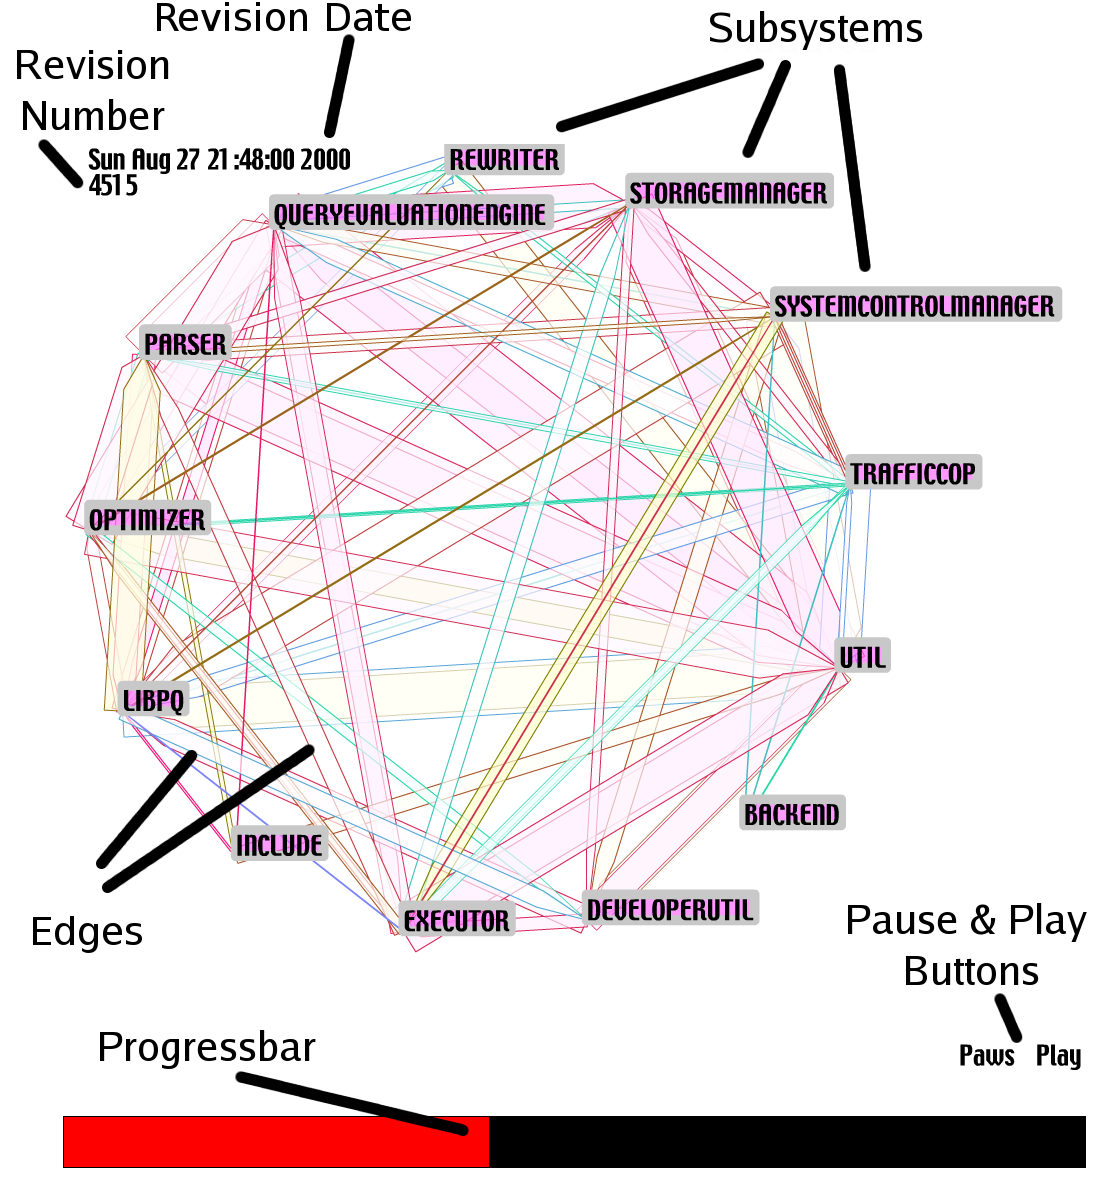
\includegraphics[height=.37\textheight]{evoflash}
\caption{Screen-shot of \YARN with \postgresql}
\label{fig:evoscreen}
\end{figure}

\addtocounter{figure}{2}
\begin{figure*}[h]
  \centering
\begin{tabular}{lr}
    \igWhs{presentation/graph4} & \igWhs{analysis2005}\\
\end{tabular}
\caption{Important architectural changes done during the last 5
years} \label{fig:pgsql05}
\end{figure*}

\end{document}
